\documentclass[
12pt,
%draft,
a4paper
]{report}
\usepackage[
top    = 2.50cm,% presumably you don't want it to be 0pt as well?
bottom = 2.50cm,
left   = 2cm,
right  = 2cm,
marginparsep = 0pt,
marginparwidth=0pt,
]{geometry}
\usepackage{textcomp}
\usepackage{standalone}
\usepackage{pgfplots}
\usepackage{draftwatermark}
\usepgfplotslibrary{fillbetween}
\usetikzlibrary{patterns}
\usepackage{commath}
%\usepackage[export]{adjustbox}
\usepackage{graphicx}
\graphicspath{{pictures/}}
\usepackage{multicol}
\usepackage[siunitx, RPvoltages]{circuitikz}
\usepackage[most]{tcolorbox}
\usepackage{varwidth}   %% provides varwidth environmen
\usepackage{amsmath,empheq}
\tcbuselibrary{skins}
\usepackage{cancel}
\newtcolorbox{mybox}[1][]{before=\centering, drop fuzzy shadow, enhanced, colback=white, sharp corners, colframe=red, fonttitle=\bfseries, title=#1, center title}
\setlength{\columnseprule}{1pt}
\usepackage{polynom}
\everymath{\displaystyle}
\makeatletter
\def\pld@CF@loop#1+{%
	\ifx\relax#1\else
	\begingroup
	\pld@AccuSetX11%
	\def\pld@frac{{}{}}\let\pld@symbols\@empty\let\pld@vars\@empty
	\pld@false
	#1%
	\let\pld@temp\@empty
	\pld@AccuIfOne{}{\pld@AccuGet\pld@temp
		\edef\pld@temp{\noexpand\pld@R\pld@temp}}%
	\pld@if \pld@Extend\pld@temp{\expandafter\pld@F\pld@frac}\fi
	\expandafter\pld@CF@loop@\pld@symbols\relax\@empty
	\expandafter\pld@CF@loop@\pld@vars\relax\@empty
	\ifx\@empty\pld@temp
	\def\pld@temp{\pld@R11}%
	\fi
	\global\let\@gtempa\pld@temp
	\endgroup
	\ifx\@empty\@gtempa\else
	\pld@ExtendPoly\pld@tempoly\@gtempa
	\fi
	\expandafter\pld@CF@loop
	\fi}
\def\pld@CMAddToTempoly{%
	\pld@AccuGet\pld@temp\edef\pld@temp{\noexpand\pld@R\pld@temp}%
	\pld@CondenseMonomials\pld@false\pld@symbols
	\ifx\pld@symbols\@empty \else
	\pld@ExtendPoly\pld@temp\pld@symbols
	\fi
	\ifx\pld@temp\@empty \else
	\pld@if
	\expandafter\pld@IfSum\expandafter{\pld@temp}%
	{\expandafter\def\expandafter\pld@temp\expandafter
		{\expandafter\pld@F\expandafter{\pld@temp}{}}}%
	{}%
	\fi
	\pld@ExtendPoly\pld@tempoly\pld@temp
	\pld@Extend\pld@tempoly{\pld@monom}%
	\fi}
\makeatother
\usepackage{wrapfig}
\usepackage{gensymb}
\makeatletter
\let\savedchap\@makechapterhead
\def\@makechapterhead{\vspace*{-3cm}\savedchap}
\usepackage{amssymb}
\usepackage{setspace}
\usepackage[norndcorners,customcolors]{hf-tikz}
\tikzset{set border color=black,set fill color=white}
\newcommand*{\qe}{$x=\frac{-b\pm\sqrt{b^2-4ac}}{2a}$}
\usepackage[linewidth=1pt]{mdframed}
\usepackage{fancyhdr}
\usepackage{array}
\usepackage[utf8]{inputenc}
\usepackage{chngcntr}
\usepackage[english]{babel}
\makeatletter
\newcommand{\leqnomode}{\tagsleft@true\let\veqno\@@leqno}
\newcommand{\reqnomode}{\tagsleft@false\let\veqno\@@eqno}
\makeatother
\usepackage{amsmath}
\usepackage{amsthm}


%Adding derivative fraction
\renewcommand\od[2]{\frac{d#1}{d#2}}

\theoremstyle{definition}
\newtheorem{example}{Example}
\counterwithin*{example}{section}
\counterwithin*{example}{subsection}


% Swap the definition of \abs* and \norm*, so that \abs
% and \norm resizes the size of the brackets, and the 
% starred version does not.
\makeatletter
\let\oldabs\abs
\def\abs{\@ifstar{\oldabs}{\oldabs*}}
%
\let\oldnorm\norm
\def\norm{\@ifstar{\oldnorm}{\oldnorm*}}
\makeatother
\usepackage{titling}
\predate{}
\postdate{}
\date{} % clear date
\pagestyle{fancy}
\rfoot{\thepage}
\cfoot{}

\setlength{\jot}{13pt}
\begin{document}
		\documentclass{standalone}
\begin{document}
\begin{titlepage} % Suppresses headers and footers on the title page
		
		\centering % Centre everything on the title page
		
		\scshape % Use small caps for all text on the title page
		
		\vspace*{\baselineskip} % White space at the top of the page
		
		%------------------------------------------------
		%	Title
		%------------------------------------------------
		
		\rule{\textwidth}{1.6pt}\vspace*{-\baselineskip}\vspace*{2pt} % Thick horizontal rule
		\rule{\textwidth}{0.4pt} % Thin horizontal rule
		
		\vspace{0.75\baselineskip} % Whitespace above the title
		
		{\LARGE Pure Mathematics\\Advanced Level} % Title
		
		\vspace{0.75\baselineskip} % Whitespace below the title
		
		\rule{\textwidth}{0.4pt}\vspace*{-\baselineskip}\vspace{3.2pt} % Thin horizontal rule
		\rule{\textwidth}{1.6pt} % Thick horizontal rule
		
		\vspace{2\baselineskip} % Whitespace after the title block
		
		%------------------------------------------------
		%	Subtitle
		%------------------------------------------------
		
		“Once your soul has been enlarged by a truth, it can never return to its original size.”\\
		-Blaise Pascal% Subtitle or further description
		
		\vspace*{3\baselineskip} % Whitespace under the subtitle
		
		%------------------------------------------------
		%	Editor(s)
		%------------------------------------------------
		
		Notes By
		
		\vspace{0.5\baselineskip} % Whitespace before the editors
		
		{\scshape\Large Giorgio Grigolo \\ } % Editor list
		
		\vspace{0.5\baselineskip} % Whitespace below the editor list
		
		\textit{Student of Mathematics and Computer Science \\St.Aloysius College } % Editor affiliation
		
		\vfill % Whitespace between editor names and publisher logo
		
		%------------------------------------------------
		%	Publisher
		%------------------------------------------------
		
		
		\vspace{0.3\baselineskip} % Whitespace under the publisher logo
		
		2020 % Publication year
		
	\end{titlepage}
	\end{document}
		
		\tableofcontents
		\newpage
	
	
		\SetWatermarkText{Giorgio G.}
		\SetWatermarkScale{5}
	
	%	\input{Class of Numbers}
	%	\documentclass{standalone}
\begin{document}
	\chapter{Surds}
	\section{Introduction}
	\quad Consider numbers $\sqrt{64}, \sqrt{16}$. These can be represented as exact quantities by writing $8$ and $4$. There are however other numbers which cannot be expressed as exact quantities using other symbols.\\
	
	
	There is an option of expressing them as corrected decimals without however preserving their full value. Instead, we choose to keep the form $\sqrt{a}$ which preserves the full value of the numbers.
	\section{Examples}
	\begin{multicols}{2}
		\noindent
		\begin{alignat*}{2}
			a)\quad
			\sqrt{2} & = \sqrt{16\times3}          \\
			& = \sqrt{16} \times \sqrt{3} \\
			& = 4\sqrt{3}                 
		\end{alignat*}
		\begin{alignat*}{2}
			b)\quad
			\sqrt{72} & = \sqrt{8\times9}         \\
			& = \sqrt{9}\times \sqrt{8} \\
			& = 3\sqrt{8}               
		\end{alignat*}
		\begin{alignat*}{2}
			\quad
			\sqrt{360} & = \sqrt{180} \times \sqrt{2} \\
			& =\sqrt{36}\times\sqrt{10}    \\
			& =6\sqrt{10}                  
		\end{alignat*}
		\begin{alignat*}{2}
			d)\quad
			& \quad\left(1+2\sqrt{3}\right)\left(2+3\sqrt{5}\right) \\
			& = 2-\sqrt{3}  - 10\sqrt{3}                            \\
			& =-28-\sqrt{3}                                         
		\end{alignat*}
		\begin{alignat*}{2}
			e)\footnote[1]\quad
			& \quad\left(2-3\sqrt{5}\right)\left(2+3\sqrt{5}\right) \\
			& = 4+6\sqrt{5}-6\sqrt{5}-9(5)                          \\
			& =-41                                                  
		\end{alignat*}
	\end{multicols}
	\footnotetext[1]{This expression shows that for products of the form $\left(a+b\sqrt{c}\right)\left(a-b\sqrt{c}\right)$ the surds will vanish.}
	\newpage
	\section{Rationalizing the denominator}
	\quad \emph{Consider the fraction:} 
	$$\frac{1}{1+\sqrt{2}}$$
	This fraction contains a surd, thus, making it irrational. To rationalize said fraction one should find the multiplicative operation of canceling the denominator \textit{(see \footnotemark[1])}.\\
	
	
	\emph{Continuing...}
	\begin{alignat*}{2}
		\frac{1}{1+\sqrt{2}} & = \frac{1}{1+\sqrt{2}} \times \frac{1-\sqrt{2}}{1-\sqrt{2}} \\
		& =\frac{1-\sqrt{2}}{1}                                       \\
		& =1-\sqrt{2}                                                 
	\end{alignat*} 
\end{document}
	%	\input{Partial Fractions}
	%	\input{Pascal tri}
	%	\input{RemFact Theroem}
	%	\input{Quadratic Equations}
	%	\documentclass{standalone}
\begin{document}
		\chapter{Logarithms}
	\section{Definition}
	\quad In mathematics, the logarithm is the inverse function to exponentiation. That means the logarithm of a given number $x$ is the exponent to which another fixed number, the base $b$, must be raised, to produce that number $x$.\\
	
	\emph{Consider: }\\$$ 2^3 = 8$$\\
	
	3 is the exponent by which 2 must be raised to obtain 8. This statement can also be reversed:\\ 3 is the logarithm by which with a base of 2, results in 8. Thus:$$ 3 = \log_28$$\\
	
	\emph{In general: }\\$$a^b = c \iff \log_ac = b ,\quad a \in \mathbb{R^+}$$\\
	
	
	Furthermore, it is standard to represent $\log_{10}(x)$ as $\log(10) $ and $ \log_e(x) $ as $ \ln(x) $
	
	
	\bigskip
	\bigskip
	\bigskip
	\bigskip
	
	\tcbset{
		enhanced,
		colback=red!5!white,
		boxrule=0.1pt,
		colframe=black!75!black,
		fonttitle=\bfseries
	}
	\begin{center}
		\begin{tcolorbox}[center title,hbox,    %%<<---- here
			lifted shadow={1mm}{-2mm}{3mm}{0.1mm}%
			{black!50!white}]
			\begin{varwidth}{\textwidth}
				\begin{center}
					$	\log_a1                         = 0                    $ \\
					\bigskip
					$\log_aa                          = 1                    $ \\
					\bigskip
					$	\log_c(ab)                       \equiv \log_ca + log_cb $\\
					\bigskip
					$	\log_c\left (\frac{a}{b}\right)  \equiv \log_ca - log_cb$ \\
					\bigskip
					$	n\log_ca                         \equiv \log_ca^n   $     
				\end{center}
			\end{varwidth}
		\end{tcolorbox} 
	\end{center}
	\section{Proofs}
	
	
	
	\paragraph{Proof 1: }$\log_aa  = 1$
	\begin{center}
		$	\text{Let} \log_aa = x$
		$$   a^x      = a $$
		$$x        =1 $$
	\end{center}
	\paragraph{Proof 2: }$\log_aa  = 1$
	\begin{center}
		$	\text{Let} \log_a1 = x$
		$$   a^x      = 1 $$
		$$x        = 0$$
	\end{center}
	\paragraph{Proof 3: }$\log_cab  = \log_ca + \log_cb$
	\begin{center}
		$	\text{Let} \log_ca = x$ ; $\text{Let} \log_cb = y$
		$$\Rightarrow  c^{x} = a  \text{ ; } c^{y} = b$$
		$$\Rightarrow ab = c $$
		$$\Rightarrow\log_c(ab) = \log_c(x) + \log_c(y)$$
		$$\therefore\quad \log_c(ab) = \log_c(a) + \log_c(b)$$
	\end{center}
	\paragraph{Proof 4: }$\log_c\frac{a}{b}  = \log_ca - \log_cb$
	\begin{center}
		$	\text{Let} \log_ca = x$ ; $\text{Let} \log_cb = y$
		$$  c^{x} = a  \text{ ; } c^{y} = b$$
		$$\frac{a}{b} = c^x \times c^{-y} $$
		$$\log_c\frac{a}{b} = \log_c(x) - \log_c(y)$$
	\end{center}
	\paragraph{Proof 5: }$\log_ca^n = n\log_ca$
	\begin{center}
		$	\text{Let} \log_ca^n = x$
		$$ c^x = a^n$$
		$$c^{\frac{x}{n}} = a  $$
		$$\log_ca = \frac{x}{n}$$
		$$x = n\log_ca $$
	\end{center}
\end{document}
	%	\documentclass{standalone}
\begin{document}
	\chapter{Vectors}
	\section{Definition}
	\quad A vector quantity is one which has magnitude and direction. For example, length is defined only by size and therefore is a \textit{scalar quantity}. However, acceleration due to gravity, while having a known magnitude, it is also acting in a particular direction. Hence, acceleration is a vector quantity.
	
	\begin{wrapfigure}{r}{0.25\textwidth}
		\includegraphics[width=1.3\linewidth]{vect_1} 
	\end{wrapfigure}
	
	Vectors are represented using line segments with arrows to denote their direction. Hence, we may consider vector $\overrightarrow{AB}$.
	
	\begin{itemize}
		\item{Two vectors are s.t.b equal iff they have the same magnitude and act in the same direction.}
		\item{The modulus refers to the size of a vector $\underline{a}$ and is denoted by $\abs{a}$.}
		\item{Two vectors $\underline{a}$ and  $-\underline{a}$  are equal in magnitude but opposite in direction. Hence the negative sign indicates opposing direction.}
		\item{When a vector is multiplied by a scalar, its magnitude changes. thus $\lambda  \underline{a}$ is a vector in the same direction as  $\underline{a}$ but has magnitude $\lambda\abs{\underline{a}}$}
	\end{itemize}
	\section{Position Vectors and Free Vectors}
	\quad When we refer to a vector  $\underline{a}$ we refer to a vector which is not confined to a specific position on the plane or in space.  $\underline{a}$, as such, is a \textit{free vector}.\\
	
	When we refer to the position vector  $\underline{b}$, we refer to a vector which is initially set to start from a specific location, usually, the origin.\\
	\setlength{\columnseprule}{0pt} 
	\begin{multicols}{2}
		\begin{center}
			\includegraphics[scale=0.16]{vect_2} 
		\end{center}
		\begin{center}
			~\\~\\~\\
			Suppose that  $\underline{a}$ and  $\underline{b}$ are non-parallel free vectors, and that the origin is a fixed point. There exists only one plane which contains the point $(0,0)$,  $\underline{a}$ and  $\underline{b}$.
		\end{center}
		
	\end{multicols}
	
	Consider another point $p$ on this plane.
	\begin{multicols}{2}
		\begin{center}
			\includegraphics[scale=0.16]{vect_2} 
		\end{center}
		\begin{itemize}
			\item{$\vec{OP}$ is the PV \footnote{Position Vector} of P}
			
			\item{	$\overrightarrow{OC}$ is $\parallel$ to $\textbf{b}$, thus $\overrightarrow{OC} = \lambda \textbf{b}$}
			\item{$\overrightarrow{CP}$ is $\parallel$ to \textbf{a}, thus $\overrightarrow{CP} = \gamma \textbf{a}$}
			\item{$\overrightarrow{OP} = \overrightarrow{OC} + \overrightarrow{PC}	 =\gamma \textbf{a} + \lambda \textbf{b}$}
		\end{itemize}
		
	\end{multicols}
	~\\
	
	Therefore, the point $O$ and the vectors \textbf{a} and \textbf{b} form a frame of reference for the position of any point on the plane. The vectors \textbf{a} and \textbf{b} are known as the base vectors. Any vector parallel to the plane can be expressed in the form $\gamma \textbf{a} + \lambda \textbf{b}$ where $\lambda$ and $\gamma$ are scalar quantities.\\
	
	
	This basis spans the usual $x$ and $y$ plane. The base vectors are \textbf{i} and \textbf{j} respectively denoting the unit base vector in the positive $x$ direction and similarly in the positive $y$ direction.\\
	
	In general, given the points $A(x_1,y_1)$ and $B(x_2,y_2)$, the vector $\overrightarrow{AB}$ is given by:	
	
	
	\begin{center}
		\begin{tcolorbox}[center title,hbox,    %%<<---- here
			lifted shadow={1mm}{-2mm}{3mm}{0.1mm}%
			{black!50!white}]
			\begin{varwidth}{\textwidth}
				\begin{center}
					$$\overrightarrow{AB} = (x_2 -x_1)\textbf{i} - (y_2 -y_1)\textbf{j}$$
					
					$$	\abs{\overrightarrow{AB}} = \sqrt{(x_2 -x_1)^2 + (y_2 -y_1)^2}$$
				\end{center}
			\end{varwidth}
		\end{tcolorbox} 
	\end{center}
	\newpage
	\section{Unit vectors}
	
	
	
	A unit vector is a vector with magnitude 1. Consider vector $\textbf{v}$ \& let $\abs{\textbf{v}}$ be its magnitude. A unit vector in the direction of $\textbf{v}$, denoted by $\hat{\textbf{v}}$ can be obtained by dividing $\textbf{v}$ by its magnitude.
	
	$$\hat{\textbf{v}} = \frac{\textbf{v}}{\abs{\textbf{v}}}$$
	
	
	\section{Vectors in 3D space}
	
	The ideas developed in the previous section can be extended to the 3-dimensional space. Thus any point $A(x_1,y_1,z_1)$ in the 3D space has position vector $\overrightarrow{OA}$.
	\begin{center}
		\begin{tcolorbox}[center title,hbox,    %%<<---- here
			lifted shadow={1mm}{-2mm}{3mm}{0.1mm}%
			{black!50!white}]
			\begin{varwidth}{\textwidth}
				\begin{center}
					$$\overrightarrow{OA} = x\textbf{i} + y\textbf{j} +z\textbf{k}$$
					$$\abs{\overrightarrow{OA} = \sqrt{x^2 + y^2 + z^2}}$$
				\end{center}
			\end{varwidth}
		\end{tcolorbox} 
	\end{center}
	
	Also, given two points $A(x_1,y_1,z_1)$ and $B(x_2,y_2,z_2)$, the vector $\overrightarrow{AB}$ is given by:
	\begin{center}
		\begin{tcolorbox}[center title,hbox,    %%<<---- here
			lifted shadow={1mm}{-2mm}{3mm}{0.1mm}%
			{black!50!white}]
			\begin{varwidth}{\textwidth}
				\begin{center}
					$$\overrightarrow{AB} = (x_2 -x_1)\textbf{i} - (y_2 -y_1)\textbf{j} + (z_2 - z_1)\textbf{k}$$
					
					$$	\abs{\overrightarrow{AB}} = \sqrt{(x_2 -x_1)^2 + (y_2 -y_1)^2 + (z_2 - z_1)^2}$$
				\end{center}
			\end{varwidth}
		\end{tcolorbox} 
	\end{center}
	
	\subsection{Direction ratios of a Vector}
	
	Given the vector $a\textbf{i}+b\textbf{j}+c\textbf{k}$, the ratios $a\colon b\colon c$ are called the direction ratios of the vector.\\
	
	Since the numbers $a$, $b$ and $c$ define the inclination of the vector in space, it follows that parallel vectors have equivalent direction vectors.\\
	
	In vectors, parallelism can be of two types:\\
	\begin{itemize}
		\item{Like parallel}
		\subitem{Two like parallel vectors both travel in the same direction.}
		\item{Unlike parallel}
		\subitem{Two unlike parallel vectors are still positionally parallel but act in the opposite direction.}
	\end{itemize}
	~\\
	In both cases, the direction ratios, however, are the same. For instance, consider the two vectors:
	
	\begin{alignat*}{2}
		&   & \textbf{a} & = 3\textbf{i} + 5\textbf{j} + 6\textbf{k}  \\
		&   & \textbf{b} & = -3\textbf{i} -5\textbf{j}  - 6\textbf{k} 
	\end{alignat*}
	Both of them will simplify to an equivalent ratio when multiplied by $-1$.
	
	\subsection{3-Dimensional Lines}
	
	Lines in 3D are better explained through vector geometry. Coordinate geometry is sufficient for the analysis of lines in 2D, however, when adding the third dimension, this becomes inefficient.
	
	\subsubsection{Equation of a straight line}
	
	The previous notion of the definition of a straight line, $y=mx+c$ or more particularly $y_2-y_1 = m(x_2-x_1)$ becomes insufficient to define a line on 3 planes of space.\\
	
	A line in 3D space is defined by a point through which it passes, and a direction to which it is parallel. Consider the following diagram:
	
	
	\begin{center}
		\includegraphics[scale=0.15]{vect_3}
	\end{center}
	
	
	Let $A$ be a fixed point on the line $l$ with position vector $\textbf{a}$ \& let $P$ represent a general point on the line. Let the position vector of $P$ be $\textbf{r}$. Consider also a vector $\textbf{m}$ parallel to the line $l$.\\
	
	We need to find the equation of line $l$, specifically, a rule defining the line $l$ which governs all points $P$ on this line. To generate the line $l$ as described above, the point $P$ must be such that $\overrightarrow{AP}$ is parallel to $\textbf{m}$.
	
	\begin{multicols}{3}
		$$	 \textbf{r}  = \textbf{a} + \lambda \textbf{m}$$
		
		\begin{alignat*}{2}
			&   & x & = x_1 + \lambda a \\
			&   & y & = y_1 + \lambda b \\
			&   & z & = z_1 + \lambda c 
		\end{alignat*}
		\begin{alignat*}{2}
			&   & x & = x_1 + \lambda a \\
			&   & y & = y_1 + \lambda b \\
			&   & z & = z_1 + \lambda c 
		\end{alignat*}
		\begin{center}
			~\\
			~\\
			$\frac{x-x_1}{a} = \frac{y-y_1}{b} = \frac{z-z_1}{c}$
		\end{center}
	\end{multicols}
	\end{document}
	%	\documentclass{standalone}
\begin{document}
	\chapter{Inequalities}
	\section{Quadratic Inequalities}
	\begin{example}
		Solve the inequality $x^2-2x>3$
	\end{example}
	
	\begin{center}
		$$x^2-2x>3$$
		$$\implies x^2-2x-3>0$$
		$$\text{Let }x^2-2x-3=0$$
		$$\implies(x-3)(x+1)=0$$
	\end{center}	
	\begin{center}
		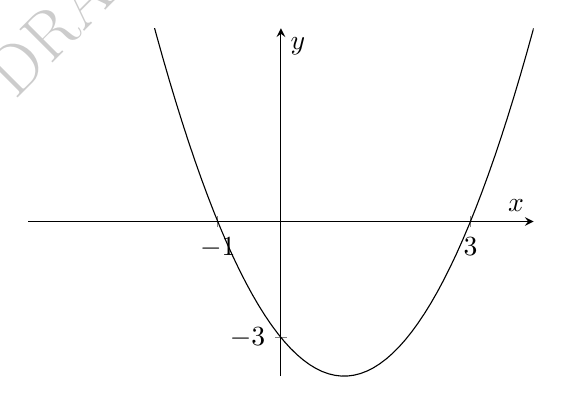
\begin{tikzpicture}
			\begin{axis}[
				width=8cm,
				height=6cm,
				axis line style={-},
				xmin=-4,
				xmax=4,
				ymin=-4,
				ymax=5,
				xtick={-1,3}, % remove all ticks from x-axis
				ytick={-3}, % ditto for y-axis
				xlabel=$x$, 
				ylabel=$y$,
				axis lines=center, % default is to make a box around the axis
				samples=100]
				\addplot [black] {x^2 - 2*x - 3}
				;
			\end{axis}
		\end{tikzpicture}
	\end{center}
	\hrulefill
	\begin{example}
		Solve the inequality $\quad \dfrac{2x^2}{5} \leq \dfrac{7x+10}{2}$
	\end{example}
	\begin{center}
		$$4x^2 \leq 35x + 50$$
		$$\implies 4x^2-35x-50\leq 0$$
		$$\text{Let }\quad 4x^2-35x-50=0$$
		$$(4x+5)(x-10)=0$$
		\begin{tikzpicture}
			\begin{axis}[
				width=8cm,
				height=6cm,
				axis line style={-},
				xmin=-2,
				xmax=11,
				ymin=-127,
				ymax=50,
				xtick={-5/4,10}, 
				ytick={-50}, 
				xlabel=$x$, 
				ylabel=$y$,
				axis lines=center, 
				samples=100]
				\addplot [black] coordinates{
					(-1,-17)(0,-48)(1,-79)(2,-110)(3,-141)(4,-172)(5,-203)(6,-234)(7,-265)(8,-296)(9,-327)(10,-358)(11,-389)	
				};
			\end{axis}
		\end{tikzpicture}
	\end{center}
	
	\hrulefill
	\end{document}
	%	\documentclass{standalone}


\begin{document}
	
	\chapter{Series}
	\section{Maclaurin Series}
	\subsection{Derivation}
	Let $f(x)$ be nay function of $ x $ and suppose that $ f(x) $ can be expanded as a series of ascending powers of $ x $ and that this series can be differentiated $ w.r.t. x $
	\begin{center}
		$	f(x) \equiv a_0   + a_{1}x  + a_{2}x^2 + a_{3}x^3 + a_{4}x^4 + ... +	 a_{r}x^r$\\
		\text{where $a_n$ are constants to be found}
	\end{center}
	Thus, inputting $0$ into $f(x)$ returns:
	$$\boxed{f(0) = a_{0}}$$\\
	Differentiating  $f(x)$ $w.r.t.x\colon$ 
	$$f'(x) \equiv a_{1} + 2a_{2}x + 3a_{3}x^2 + 4a_4x^3 + \cdots + ra_{r}x^{r-1} + \cdots$$
	Inputting $0$ into $f'(x)\colon$
	$$\boxed{f'(0) = a_1}$$\\
	Differentiating $f'(x)$ $w.r.t.x\colon$
	$$f''(x) \equiv 2a_{2} + 6a_{3}x + 12a_4x^2 + \cdots + (r-1)(r)a_{r}x^{r-2} + \cdots$$
	Inputting $0$ into $f''(x)\colon$
	$$\boxed{f''(0) = 2a_2}$$\\
	Differentiating $f''(x)$ $w.r.t.x\colon$
	$$f'''(x) \equiv 6a_{3} +24a_4x + \cdots + (r-2)(r-1)(r)a_{r}x^{r-3}+ \cdots$$
	Inputting $0$ into $f'''(x)\colon$
	$$\boxed{f'''(0) = (2)(3)a_3}$$
	$$\vdots$$
	\newpage
	By the above calculation we can conclude that: 
	$$\boxed{a_r = \frac{f^r(x)}{r!}}$$
	Considering all of the above: 
	
	\tcbset{
		enhanced,
		colback=red!5!white,
		boxrule=0.1pt,
		colframe=black!75!black,
		fonttitle=\bfseries
	}
	\begin{center}
		\begin{tcolorbox}[center title,hbox,    %%<<---- here
			lifted shadow={1mm}{-2mm}{3mm}{0.1mm}%
			{black!50!white}]
			\begin{varwidth}{\textwidth}
				\begin{center}
					$f(x) \equiv f(0) + f'(0)x + \dfrac{f''(0)x^2}{2!} + \dfrac{f'''(0)x^3}{3!} + \cdots + \dfrac{f^r(0)x^r}{r!} + \cdots$\\
					\bigskip
					$\displaystyle \therefore \quad f(x) \equiv \sum_{r=1}^{\infty} \dfrac{f^r(x)}{r!}$
				\end{center}
			\end{varwidth}
		\end{tcolorbox} 
	\end{center}
	
	
	This is known as Maclaurin's Theorem, and can be obtained if and only if $f^r(0) \in \mathbb{R}$. In the following examples we use Maclaurin's Theorem to obtain the series expansion of some standard equations. The range of validity of each expansion is left as an exercise to the reader.
	\subsection{Examples}
	\begin{example}
		\emph{Express} $e^x$ \emph{as a series expansion using the Maclaurin theorem.}
	\end{example}
	Let $f(x) = e^x$
	\begin{alignat*}{5}
		&   & f(x)    & = & e^x \quad & \Rightarrow\quad & f(0) = 1    \\
		&   & f'(x)   & = & e^x \quad & \Rightarrow\quad & f'(0) = 1   \\
		&   & f''(x)  & = & e^x \quad & \Rightarrow\quad & f''(0) = 1  \\
		&   & f'''(x) & = & e^x \quad & \Rightarrow\quad & f'''(0) = 1 
	\end{alignat*}
	
	$$\therefore \quad e^x  = 1 + x + \frac{x^2}{2!} + \frac{x^3}{3!} + \frac{x^4}{4!} +\ldots + \frac{x^r}{r!} + \ldots $$
	\hrulefill
	\begin{example}
		\emph{Express} $\cos x$ \emph{as a series expansion using the Maclaurin theorem.}
	\end{example}
	\begin{alignat*}{5}
		&   & f(x)    & =           & \cos (x) \quad & \Rightarrow\quad & f(0) = 1    \\
		&   & f'(x)   & = \text{ -} & \sin (x) \quad & \Rightarrow\quad & f'(0) = 1   \\
		&   & f''(x)  & = \text{ -} & \cos(x) \quad  & \Rightarrow\quad & f''(0) = 1  \\
		&   & f'''(x) & =           & \sin (x) \quad & \Rightarrow\quad & f'''(0) = 1 
	\end{alignat*}
	$$\therefore \quad \cos (x)  = 1 - \frac{x^2}{2!} + \frac{x^4}{4!} -\frac{x^6}{6!}+\ldots + (-1)^r\times\frac{x^{2r}}{2r!} + \ldots $$\\
	The above expansion justifies the fact that when $x$ is very small and thus high powers of $x$ may be neglected, then: \boxed{\cos x \approx 1- \frac{x^2}{2}}\\
	\begin{example}
		\emph{Express} $\ln(1+x)$ \emph{as a series expansion using the Maclaurin theorem.}
	\end{example}
	
	\begin{alignat*}{5}
		&   & f(x)    & = & \ln(1+x)      \quad & \Rightarrow  \quad & f(0)    & = 0  \\
		&   & f'(x)   & = & (x+1)^{-1} \quad    & \Rightarrow  \quad & f'(0)   & = 1  \\
		&   & f''(x)  & = & -(1+x)^{-2}  \quad  & \Rightarrow \quad  & f''(0)  & = -1 \\
		&   & f'''(x) & = & 2(1+x)^{-3} \quad   & \Rightarrow  \quad & f'''(0) & = 2  
	\end{alignat*}
	$$\therefore \quad \ln(1+x)  = x - \frac{x^2}{2} + \frac{x^3}{3} - \ldots + (-1)^{r+1}\times\frac{x^r}{r} + \ldots $$\\
	\hrulefill
	
	\begin{example}
		\emph{Expand} $\arcsin(x)$ \emph{up to the term in $x^3$. By putting $x=\frac{1}{2}$, find an approximate value for $\pi$}
	\end{example}
	
	\begin{alignat*}{5}
		& f(x)    & = & \arcsin(x)      \quad                                   & \Rightarrow  \quad & f(0)    & = 0 \\
		& f'(x)   & = & (1-x^2)^{\frac{-1}{2}} \quad                            & \Rightarrow  \quad & f'(0)   & = 1 \\
		& f''(x)  & = & x(1-x^2)^{\frac{-3}{2}}\quad                            & \Rightarrow \quad  & f''(0)  & = 0 \\
		& f'''(x) & = & 3x(1-x^2)^{\frac{-5}{2}} + (1-x^2)^{\frac{-3}{2}} \quad & \Rightarrow  \quad & f'''(0) & = 1 
	\end{alignat*}
	$$\therefore \quad \arcsin(x)   = x + \frac{x^3}{3!} + \ldots $$\\
	Putting $x = \frac{1}{2}$\\
	\begin{alignat*}{2}
		&          & f\left(\frac{1}{2}\right) & = \frac{\pi}{6}                                \\
		& \implies & \pi                       & \approx 6\left(\frac{1}{2}+\frac{1}{81}\right) \\
		& \implies & \pi                       & \approx \frac{83}{27}                          
	\end{alignat*}
	\newpage
	\subsection{Expanding compound functions using standard functions}
	\begin{example}
		Expand $a)\quad \dfrac{e^{2x}+ e^{-3x}}{e^x}\quad b)\quad \ln\left( \dfrac{1-2x}{(1+2x)^2}\right)  $as series of ascending powers of $x$ up to the term in $x^4$. Give the general term in each case and the range of values of $x$ for which each expansion is valid.
	\end{example}
	\begin{alignat*}{2}
		a) &                  & e^x                                    & = 1 + x + \frac{x^2}{2!} + \frac{x^3}{3!} + \frac{x^4}{4!} +\ldots                                                                                                  \\
		&                  & e^{-3x}                                & = 1 + (-3)x + \frac{(-3x)^2}{2!} + \frac{(-3x)^3}{3!} + \frac{(-3x)^4}{4!} +\ldots                                                                                  \\
		& \therefore \quad & e^{x} + e^{-3x}                        & = \left (1 + x + \frac{x^2}{2!} + \frac{x^3}{3!} + \frac{x^4}{4!}\right ) + \left (1 + (-3)x + \frac{(-3x)^2}{2!} + \frac{(-3x)^3}{3!} + \frac{(-3x)^4}{4!}\right ) \\
		&                  &                                        & = 2 -2x + \frac{10x^2}{2!} - \frac{26x^3}{3!} + \frac{89x^4}{4!}                                                                                                    \\
		\bigskip\\
		b) &                  & \ln\left(\dfrac{1-2x}{(1+2x)^2}\right) & = \ln(1-2x) -2\left (\ln(1+2x)\right)                                                                                                                               
		\intertext{\emph{Consider $\ln(1-2x)\colon$}}
		&                  & \ln\left(1+(-2x)\right)                & = -2x + -2x^2-\frac{8x^3}{3}-4x^4 + \ldots + \frac{(-1)^{r-1}(-2x)^r}{r}+ \ldots                                                                                    \\
		\intertext{\emph{Consider $\ln(1+2x)\colon$}}
		&                  & \ln\left(1+2x\right)                   & = 2x + -2x^2+\frac{8x^3}{3}-4x^4 +\ldots + \frac{-2(-1)^{r-1}(2x)^r}{r} + \ldots                                                                                    \\ 
		& \therefore       & \ln\left(\dfrac{1-2x}{(1+2x)^2}\right) & = \left( -2x + -2x^2-\frac{8x^3}{3}-4x^4\right) -2\left(2x + -2x^2+\frac{8x^3}{3}-4x^4\right)                                                                       \\
		&                  &                                        & = -6x+2x^2-8x^3	+4x^{4}                                                                                                                                             \\
	\end{alignat*}
	\text{Rage of Validity:}
	\begin{multicols}{2}
		\begin{center}
			$$	\quad\frac{(-1)^{r-1}(-2x)^r}{r} - \frac{2(-1)^{r-1}(2x)^r}{r}$$\\
			$$  =\frac{(-1)^{r-1}(-1)^r(2x)^r+2(-1)^r(2x)^r}{r}$$\\
			$$	=\frac{(-1)^{2r-1}(2x)+2(-1)^r(2x)^r}{r}$$\\
			$$	=\frac{\left( (-1)^{2r-1}+2(-1)^r\right) (2x)^r}{r}$$\\
			$$  =\frac{ \left(-1+2(-1)^r\right(2x)^r)}{r}$$
			$$ =\frac{2^r(2(-1)^r -1)x^r}{r}$$							
		\end{center}
	\end{multicols}
	
	\begin{example}
		Expand  $\ln\left(\frac{x+1}{x}\right)\quad$as series of ascending powers of $x$ up to the term in $x^4$. Give the general term in each case and the range of values of $x$ for which each expansion is valid.
	\end{example}
	
	$$f(x) \ln\left(\frac{x+1}{x}\right)  = \ln\left(1+\frac{1}{x}\right ) $$
	
	\begin{alignat*}{5}
		&   & f(x)    & = & \ln(1+\frac{1}{x})    \quad & \Rightarrow  \quad & f(0)    & = 0  \\
		&   & f'(x)   & = & (x+1)^{-1} \quad            & \Rightarrow  \quad & f'(0)   & = 1  \\
		&   & f''(x)  & = & -(1+x)^{-2}  \quad          & \Rightarrow \quad  & f''(0)  & = -1 \\
		&   & f'''(x) & = & 2(1+x)^{-3} \quad           & \Rightarrow  \quad & f'''(0) & = 2  
	\end{alignat*}
	
	\begin{center}
		$=\frac{1}{x} - \frac{1}{2x^2} + \frac{1}{3x^3} - \frac{1}{4x^4} + \ldots + \frac{(-1)^{r+1}}{r} $
	\end{center}
	\hrulefill
	\begin{example}
		Expand $\sin^2{x}$ using Maclaurin's series up to $x^4$
	\end{example}
	\bigskip
	$$sin^2(x)\equiv\frac{1-\cos(2x)}{2}$$
	\begin{alignat*}{2}
		\intertext{\emph{Consider} $\cos(2x)\colon$} &                 &           & =1-\frac{(2x)^{2}}{2!} + \frac{(2x)^4}{4!}  - \cdots + \frac{(-1)^r(2x)^{2r}}{(2r)!}+\cdots           \\
		&                 &           & =1-2x^2+\frac{2x^4}{3}-\cdots+\frac{(-1)^r(2x)^{2r}}{(2r)!}+\cdots                                    \\
		& \therefore\quad & \sin^2(x) & \equiv \frac{1}{2}\left( 1-(1-2x^2+\frac{2x^4}{3}-\cdots+\frac{(-1)^r(2x)^{2r}}{(2r)!}+\cdots)\right) \\
		&                 &           & =\frac{1}{2}\left(1-1+2x^2 - \frac{2x^4}{3} +\cdots+\frac{(-1)^r(2x)^{2r}}{(2r)!}+\cdots\right)       \\
		&                 &           & =x^2-\frac{x^4}{3} +\cdots+\frac{(-1)^{r+1}(2x)^{2r}}{(2r)!}+\cdots                                   
	\end{alignat*}
	\newpage
	\begin{example}
		Given $e^{2x}\cdot \ln{1+ax}$ find possible values for $p$ and $q$.
	\end{example}
	\begin{alignat*}{2}
		\intertext{\emph{Consider} $e^{2x}\colon$}
		&                 & e^{2x}                & = 1+2x + \frac{(2x)^2}{2!} + \frac{(2x)^{3}}{3!} +\cdots +  \frac{x^r}{r!} + \cdots           \\
		\intertext{\emph{Consider} $\ln(1+ax)\colon$}
		&                 & \ln(1+ax)             & = ax - \frac{(ax)^2}{2} + \frac{(ax)^3}{3} - \cdots + \frac{(-1)^{r+1}x^r}{r} + \cdots        \\
		& \therefore\quad & e^{2x}\cdot \ln(1+ax) & = \left(1+2x+2x^2+\frac{4x^3}{3}\right) \left(ax - \frac{a^2x^2}{2} + \frac{a^3x^3}{3}\right) \\
		&                 &                       & =ax-\frac{a^2x^2}{2}+\frac{a^3x^3}{3}+2ax^2-2a^2x^3                                           \\
		&                 &                       & =ax-\left(\frac{a^2}{2}+2a\right) x^2+\left( \frac{a^3}{3}-2a^2\right) x^3                    
	\end{alignat*}
	~\\
	\begin{equation*}
		\therefore\left.
		\begin{alignedat}{2}
			\hspace{0.5 in}	&&p&=a\\
			&&	\frac{a^2}{2}+2a&=\frac{-3}{2}\\
			&&	\frac{a^3}{3}-2a^2&=q
		\end{alignedat}	\right\}
	\end{equation*}
	
	\begin{center}
		$$ p = -3,-1 $$
		$$ q= -27, -\dfrac{7}{3}$$
	\end{center}
	\hrulefill
	\newpage
	\section{Summation of Series}
	\subsection{Method 1: Generating differences}
	
	\begin{example}
		Simplify $f(r)-f(r+1)$, when $f(x) = \frac{1}{r^2}$. Hence, find the sum up to $n$ terms of:\\ $$\sigma_1 = \frac{3}{1^2\cdot 2^2} + \frac{5}{2^2\cdot 3^2} + \frac{7}{3^2\cdot 4^2} + \ldots$$
	\end{example}
	~\\
	Simplifying $f(r) - f(r+1)\colon$
	\begin{alignat*}{2}
		&   & f(r)-f(r+1) & = \frac{1}{r^{2}} - \frac{1}{(r+1)^{2}} \\
		&   &             & =\frac{(r+1)^{2}-r^2}{r^2(r+1)^{2}}     \\
		&   &             & =\frac{2r+1}{r^2(r+1)^2}                
	\end{alignat*}
	\textit{Generating series and adding}\\
	\textit{quantitatively equivalent terms:}
	\begin{center}
		$	\frac{1}{1^2} - \cancel{\frac{1}{2^2}}$
		$$	\cancel{\frac{1}{2^2}} - \cancel{\frac{1}{3^2}}$$
		$$	\cancel{\frac{1}{3^2}} - \cancel{\frac{1}{4^2}}$$
		$$\vdots$$
		$$\cancel{\frac{1}{n^2}} - \frac{1}{n+1^2}$$
		~\\
		$$\boxed{\therefore \quad \sigma_1 = 1 - \frac{1}{n+1^2}}$$
	\end{center}
	\hrulefill
	\begin{example}
		If $f(r) = r(r+1)!$ simplify $f(r) - f(r-1)$. Hence sum the series:\\
	\end{example}
	\begin{center}
		$\sigma_1 = 5\cdot 2! + 10\cdot 3! + 17\cdot 4! +  ... + (n^2=1)n!$\\
	\end{center}
	\hrulefill
	\begin{alignat*}{2}
		&   & f(r)-f(r-1) & =r(r+1)! - (r-1)r!  \\
		&   &             & =r(r+1)r! - (r-1)r! \\
		&   &             & =r!(r^2+r-r+1)      \\
		&   &             & =r!(r^2+1)          
	\end{alignat*}
	\newpage
	\textit{Generating series and adding}\\
	\textit{quantitatively equivalent terms:}
	\begin{center}
		$\bcancel{f(2)} - f(1)$
		$$\bcancel{f(3)} - \bcancel{f(2)}$$
		$$\bcancel{f(4}) - \bcancel{f(3)}	$$
		$$\vdots$$
		$$\bcancel{f(n-1)} - \bcancel{f(n-2)}$$
		$$f(n) - \bcancel{f(n-1)}$$\\
	\end{center}
	\begin{example}
		If $f(r) = \cos2r\theta$, simplify $f(r) - f(r+1)$. Hence find $\sin3\theta + \sin5\theta + \sin7\theta$
		\hrulefill
	\end{example}
	\begin{alignat*}{2}
		&   & f(r)-f(r+1) & =\cos(2r\theta)- \cos(2(r+1)\theta)                                                                            \\
		&   &             & =-2\sin\left(\frac{2r\theta + (2r+2)\theta}{2}\right)\cdot \sin\left(\frac{ 2r\theta - 2(r+1)\theta}{2}\right) \\
		&   &             & =-2\sin(2r\theta+ \theta)\sin(-\theta)                                                                         \\
		&   &             & =2\sin(\theta[2r+1])\sin\theta                                                                                 
	\end{alignat*}
	\textit{Generating series and adding}\\
	\textit{quantitatively equivalent terms:}\\
	\begin{center}
		
		\begin{tabular}{ccccc}
			$r=1$    &   & $2\sin(3\theta)\sin(\theta)$ & $=$ & $f(1)\cancel{-f(2)}$          \\
			$r=2$    &   & $2\sin(5\theta)\sin(\theta)$ & $=$ & $\cancel{f(2)}\cancel{-f(3)}$ \\
			$r=3$    &   & $2\sin(7\theta)\sin(\theta)$ & $=$ & $\cancel{f(3)}\cancel{-f(4)}$ \\
			$\vdots$ &   & $\vdots$                     & $=$ & $\vdots$                      \\
			$r=n$    &   & $2\sin(2n+1)\sin(\theta)$    & $=$ & $\cancel{f(n)}-f(n+1)$        
		\end{tabular}\\
		~\\
		\begin{alignat*}{2}
			&   & f(1) - f(n+1) & = 2\sin(\theta)\sin(2n+1)                                \\
			&   &               & =\frac{\cos(2\theta)- \cos(2\theta(n+1))}{2\sin(\theta)} \\
			&   &               & =\frac{2\sin(\theta(2r+1))\sin\theta}{2\sin(\theta)}     \\
			&   &               & =\frac{sin((n=1)\theta)\sin(n\theta)}{\sin(\theta)}      
		\end{alignat*}
	\end{center} 
	
	
	\subsection{Method 2: Using partial fractions}
	A special case of the previous method can happen to imply a partial fraction decomposition.
	
	\begin{example}
		Decompose $\frac{1}{r(r+1)}$. Hence find the sum of $$\sigma_1 = \frac{1}{1\cdot 2} + \frac{1}{2\cdot 3} + \frac{1}{3\cdot 4} + \cdots$$
	\end{example}~\\
	\textit{Decomposing:}
	$$\frac{1}{r(r+1)} \equiv \frac{1}{r} - \frac{1}{r-1}$$
	{Generating series and adding}\\
	{quantitatively equivalent terms:}\\
	\begin{center}
		\begin{tabular}{ccccc}
			$r=1$    &   & $\frac{1}{1}$          & $-$ & $\cancel{\frac{1}{2}}$\linebreak \\
			&&&\\
			$r=2$    &   & $\cancel{\frac{1}{2}}$ & $-$ & $\cancel{\frac{1}{3}}$           \\
			&&&\\
			$r=3$    &   & $\cancel{\frac{1}{3}}$ & $-$ & $\cancel{\frac{1}{4}}$           \\
			&&&\\
			$\vdots$ &   & $\cancel{\vdots}$      & $-$ & $\cancel{\vdots}$                \\
			&&&\\
			$r=n$    &   & $\cancel{\frac{1}{n}}$ & $-$ & $\frac{1}{n+1}$                  \\
		\end{tabular}\\
	\end{center}
	\begin{alignat*}{2}	
		& \therefore \quad & \sigma_1 & = 1 - \frac{1}{n+1}                                  \\
		\intertext{Finding convergent value: }
		&                  & 1        & =\lim_{x \to \infty} \left( 1 - \frac{1}{n+1}\right) 
	\end{alignat*}
	\hrulefill
	\newpage
	\begin{example}
		Find $\quad \sum_{r=3}^n \frac{2}{(r-1)(r+1)}$
	\end{example}
	\begin{alignat*}{2}	
		\intertext{Consider $\frac{2}{(r-1)(r+1)}\colon$}
		&   & \frac{2}{(r-1)(r+1)}                                      & \equiv \frac{1}{r-1} - \frac{1}{r+1}                           \\
		&   & \therefore \quad \sum_{r=3}^n \dfrac{2}{(r-1)(r+1)} \quad & \equiv \quad  \sum_{r=3}^n \dfrac{1}{(r-1)} - \dfrac{1}{(r+1)} \\
	\end{alignat*}
	{Generating series and adding}\\
	{quantitatively equivalent terms:}\\
	\subsection{Method 3: Using standard results}
	
	\subsection{Method 4: Comparing to standard results}
	
\end{document}
	%	\input{Complex Numbers}
			\documentclass{standalone}
\begin{document}
	\chapter{Integration}
	\section{Reduction Formul\ae}
	
	\begin{example}
		If $I_n = \int \cos^n x \, dx$ show that $I_n = \frac{1}{n} \sin\cos^{n-1}x + \frac{n-1}{n}\cdot I_{n-2}$. Hence find $\int \cos^5x\, dx$.
	\end{example}
	
	\begin{align*}
							I_n  & = \int \cos^n x \, dx\\
								 & = \int \cos x \cdot \cos^{n-1}x\, dx\\
								 \text{Integrating by parts: }\\
			\therefore \quad I_n & = \cos^{n-1}x\sin x + (n-1)\int\cos^{n-2}x\sin^2x\,dx\\
								 & = \cos^{n-1}x\sin x + (n-1)\int\cos^{n-2}x(1-\cos^2x)\,dx\\
								 & = \cos^{n-1}x\sin x + (n-1)\int\cos^{n-2}x(1-\cos^2x)\,dx\\
	\end{align*}
	\begin{align*}
			\int \cos^5 x \, dx  & = I_5\\
							  	 & I_5 = \frac{1}{5} \cos^4x\sin x + \frac{4}{5}I_3\\
		& I_3 = \frac{1}{5} \cos^4x\sin x + \frac{4}{5}I_3\\
		& I_1 = \int \cos x \, dx = \sin x + k\\
		\therefore \int \cos^5 x & = \frac{1}{5}\cos^4x \sin x + \frac{4}{5}\left(\frac{1}{3}\cos^2x\sin x + \frac{2}{3}\left(\sin x + k\right)\right)\\
		& =\frac{1}{5}\cos^2x\cdot\sin x + \frac{4}{15} \cos^2 x \cdot \sin x + \frac{8}{15}\sin x + c                        
	\end{align*}	  						
	
	\begin{example}
		If $I_n = \int \tan^n\theta \, d\theta$
	\end{example}
	
	\begin{example}
		Establish a reduction formula that could be used to find $\int x^ne^x \, dx$ and use it to find $\int x^4e^4$.
	\end{example}
	
	\begin{align*}
		\text{Let } I_n & = \int x^ne^x \, dx \\
		\text{Let } u & = x^n      & \od{v}{x} = e^x \\
		\od{u}{x}     & = nx^{n-1} & v = e^x         \\
		\therefore I &= x^ne^x - n \int x^{n-1}e^x \, dx\\
		&= x^ne^x - nI_{n_{1}}
	\end{align*}
	
	\begin{example}
		Establish a reduction formula which can be used to evaluate $\int x^n \sin x \, dx$.
	\end{example}
	
	\begin{align*}
		\text{Let } I_n &= \int x^n \cdot \sin x\\
		\text{Let } u & = x^n      & \od{v}{x} = \sin x \\
		\od{u}{x}     & = nx^{n-1} & v= -\cos x         
	\end{align*}
	
	\begin{example}
		Establish a reduction formula to find $\int \csc^nx \, dx$. Hence find $\int csc^5x \, dx$
	\end{example}
	\begin{align*}
		\text{Let } I_n &= \int \csc^nx \, dx\\
		&= \int \csc^2x \cdot \csc^{n-2}x \, dx\\
		\text{Let } u & = \csc^{x-2} x              & \od{v}{x} = \csc^2x \, dx \\
		\od{u}{x}     & = -(n-2)\csc^{n-2}\cot x  v & = -\cot x                 \\
		\therefore \int \csc^nx \, dx &= -\cot x \cdot \csc^{n-2}x  - (n-2)\int \csc^{n-2}x\cot^2x \, dx\\
		I_n &= 	-\cot x \cdot \csc^{n-2}x - (n-2)\int \csc^{n-2}x\left(\csc^2x - 1\right) \, dx\\
		&= 		-\cot x \cdot \csc^{n-2}x - (n-2)\int \csc^{n-2}x\left(\csc^2x - 1\right) \, dx\\
	\end{align*}
\end{document}
	%	\input{Applications of Calculus}
\end{document}